\documentclass[aspectratio=169]{beamer} % 16:9 aspect ratio for modern screen
% \documentclass[handout]{beamer} % 16:9 aspect ratio for modern screen

% Theme settings
\usetheme[progressbar=foot]{metropolis} % Minimalist theme
\metroset{progressbar=frametitle} % Progress bar soll nur folien mit titel berücksichtigen?
\setbeamercolor{background canvas}{bg=white} % White background color

\makeatletter
    \setlength{\metropolis@progressinheadfoot@linewidth}{1.5pt}
\makeatother


\usefonttheme{professionalfonts} % Font theme

% Packages
\usepackage[T1]{fontenc}   % Font encoding
\usepackage[ngerman]{babel} % German language
\usepackage[sfdefault]{FiraSans} % For FiraSans font
\usepackage[backend=biber, style=authoryear-comp
, sorting=nyt]{biblatex} % For bibliography
\usepackage{csquotes} % Recommended for biblatex with babel/polyglossia
\usepackage{textgreek} % Greek letters in text mode (aus references von Citavi)
\usepackage{tikz}          % For drawing graphics

\usepackage{graphicx}       % For including images
\usepackage{amsmath, amssymb} % For math symbol

\usepackage[labelformat=empty]{caption}


% Bibliography settings
\addbibresource{references.bib} % Path to the bibliography file

% custom Citation commands
\DeclareCiteCommand{\citeauthortitle}
  {\usebibmacro{prenote}}
  {\usebibmacro{citeindex}%
   \printnames{labelname}%
   \setunit{\space\textendash\space}
   \printfield{title}}
  {\multicitedelim}
  {\usebibmacro{postnote}}

  \DeclareCiteCommand{\citeauthortitleurl}
  {\usebibmacro{prenote}}
  {\usebibmacro{citeindex}%
   \printnames{labelname}%
   \setunit{\space\textendash\space}
   \printfield{title}%
   \setunit{\addsemicolon\space}
   \printfield{url}}
  {\multicitedelim}
  {\usebibmacro{postnote}}

\DeclareCiteCommand{\parenciteauthortitle}
  {\usebibmacro{prenote}}
  {\bibopenparen\usebibmacro{citeindex}%
   \printnames{labelname}%
   \setunit{\space\textendash\space}% <- Hier wird das Trennzeichen ":" hinzugefügt
   \printfield{title}\bibcloseparen}
  {\multicitedelim}
  {\usebibmacro{postnote}}

\makeatletter
\renewcommand\footnotesize{\tiny}
\makeatother

\newcommand{\figcite}[1]{\\[-3mm]{\tiny Quelle: \cite{#1}}}
\newcommand{\figciteweb}[1]{\\[-3mm]{\tiny aus: \citeauthortitle{#1}}}
\newcommand{\figciteweburl}[1]{\\[-3mm]{\tiny aus: \citeauthortitleurl{#1}}}
  
\mode<handout>{
    \AtBeginSection[]{} % In Handout-Version keine Section-Folie erzeugen
}

% Title page settings
\title{Second- \& Third-Harmonic Generation}
\subtitle{Frequenzverdopplung in der nichtlinearen Optik}
\author{Florian Marius Adamczyk}
\date{07.07.2025}
\institute{Justus-Liebig-Universität Gießen \\ M.Sc. Modul \textbf{Spektroskopie} bei \textbf{PD Dr. Arash Rahimi-Iman, Dipl.-Ing.}\\ }
\titlegraphic{\vspace{-1cm}
\includegraphics[height=1.2cm]{Images/jlu_logo.jpg}}

\begin{document}

    % Black slide
    \begin{frame}<handout:0>[plain, noframenumbering]
        \begin{tikzpicture}[remember picture, overlay]
          \fill[black] (current page.south west) rectangle (current page.north east);
        \end{tikzpicture}
        \pause
        .
        \pause
        \centering
        \only<3>{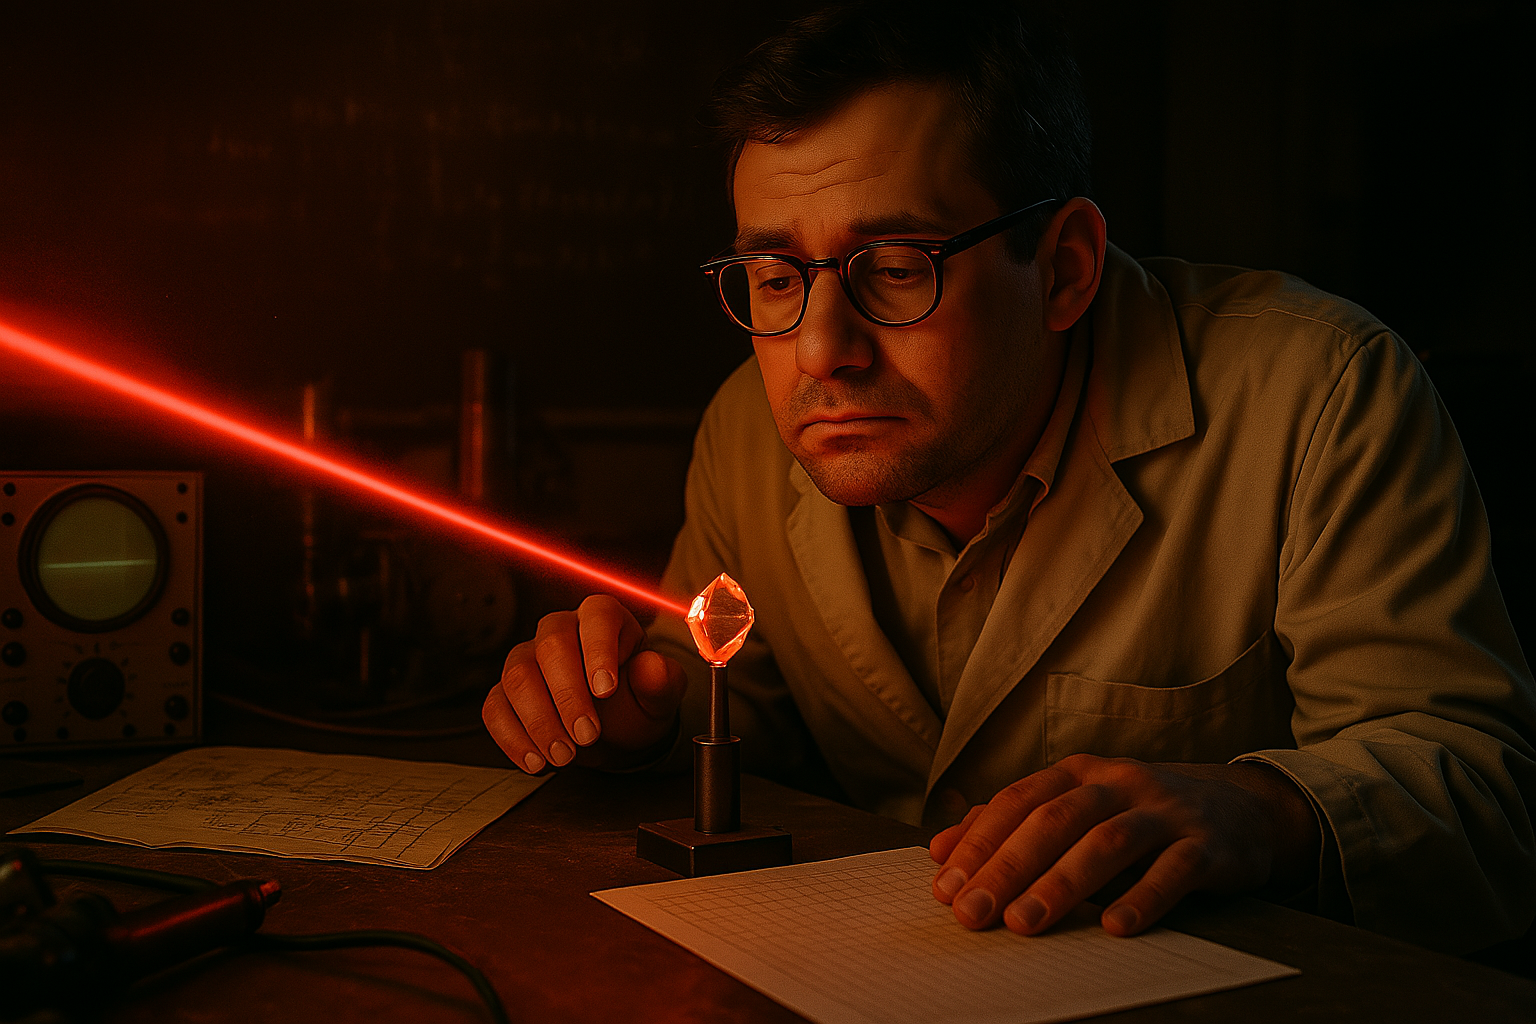
\includegraphics[width=0.9\textwidth]{Images/Copilot_20250706_224005.png}}
        \only<4>{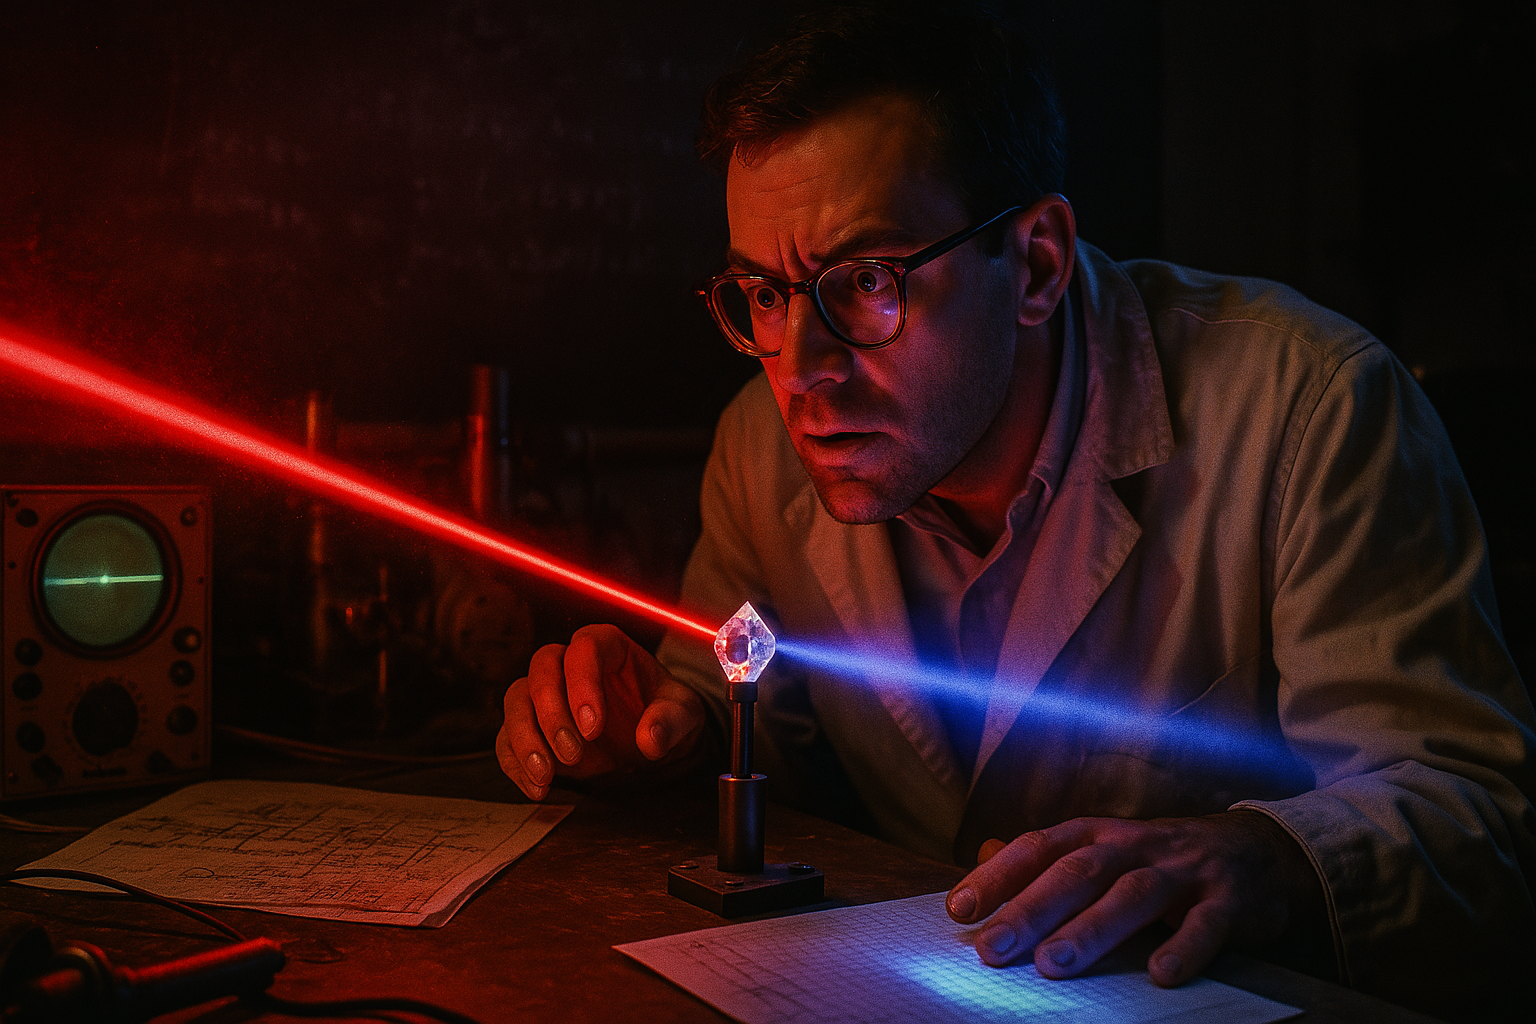
\includegraphics[width=0.9\textwidth]{Images/Copilot_20250706_215901.png}}
        \\ \tiny \textcolor{gray}{von: \citetitle{Copilot.2025} -- \citefield{Copilot.2025}{note}}
    \end{frame}
    % 1961 beobachteten der Physiker Peter Franken und seine Mitarbeiter an der University of Michigan einen merkwürdigen Effekt: Bei der Bestrahlung eines Quarzkristalls mit einem der ersten Rubinlaser bestand das transmittierte Licht nicht nur aus Strahlung der Laserwellenlänge 694 nm, sondern es trat auch UV-Licht der halben Wellenlänge 347 nm aus. Das war die erste Beobachtung eines nichtlinearen Effektes, der Frequenzverdopplung,[2] und gilt als die Geburtsstunde der nichtlinearen Optik.

    % % Appetizer Slide
    % \begin{frame}<handout:0>[noframenumbering, plain]{Appetizer}
    %     \centering
    %     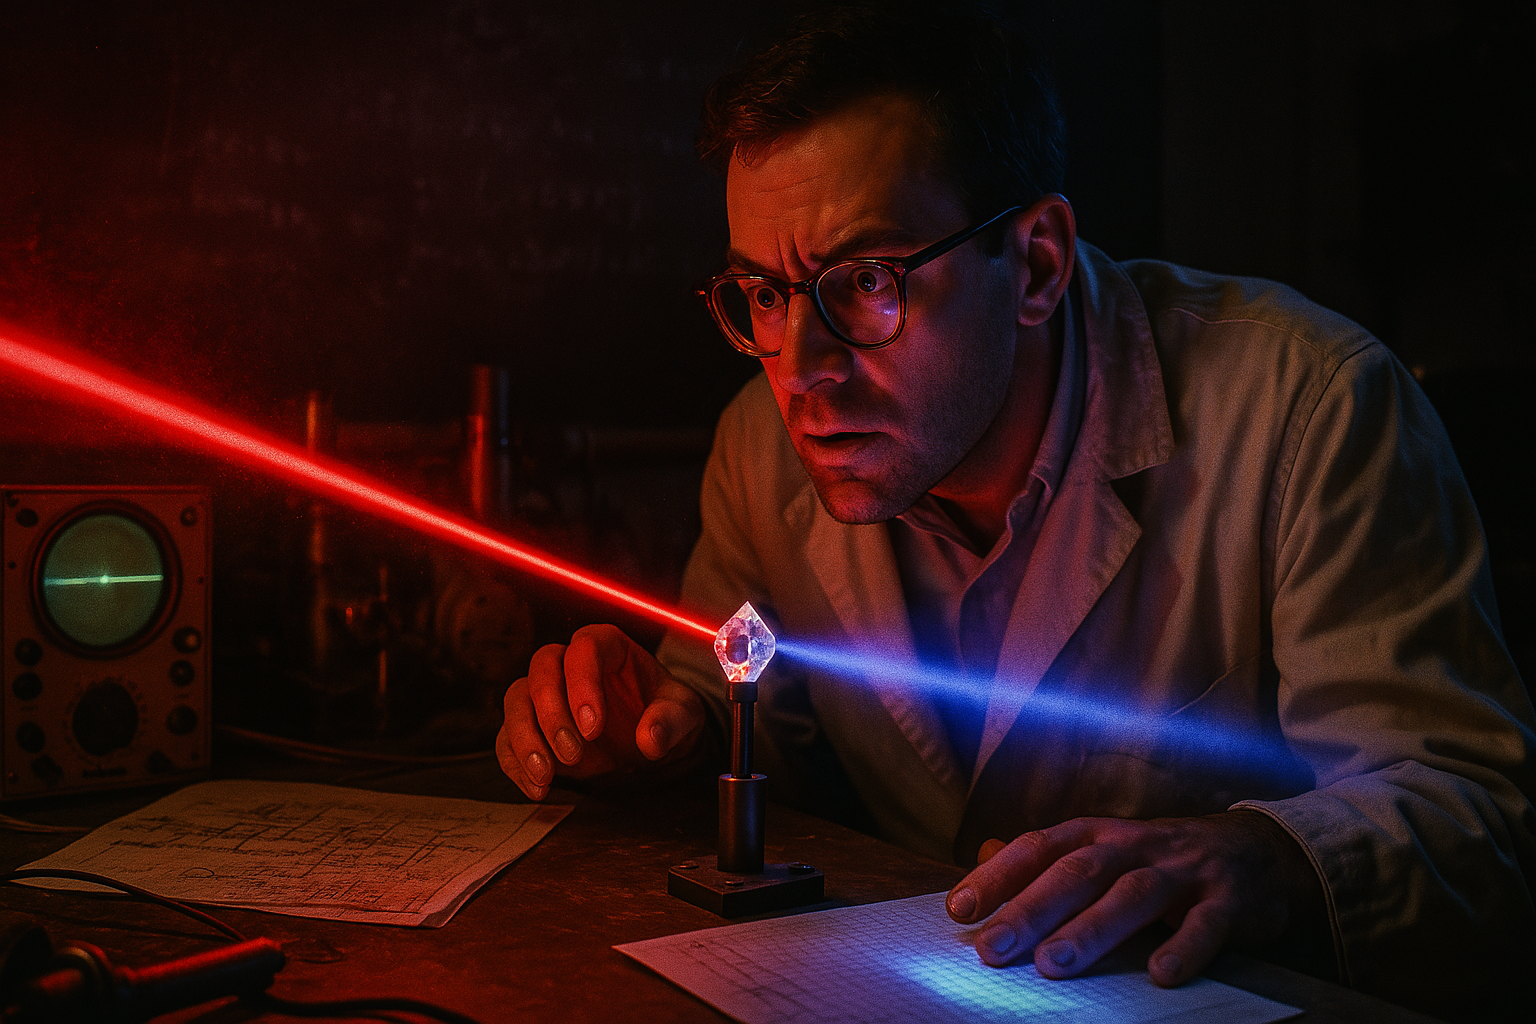
\includegraphics[width=\textwidth, height=0.9\textheight, keepaspectratio]{Images/Copilot_20250706_215901.png}
    %     \figciteweburl{Copilot.2025}
    %     % \vspace{0.5cm}
    %     % \begin{quote}
    %     %{Stellen Sie sich vor, ...}
    %     % \end{quote}
    % \end{frame}

    % Title Slide
    \begin{frame}[noframenumbering, plain]
        \vspace*{-0.6cm}
        \titlepage
        \vspace*{-1.6cm}
    \end{frame}
    
    % Table of Contents
    \begin{frame}<handout:0>{Gliederung} % Handout ausgeschaltet!!
      \setcounter{page}{1}      
        \tableofcontents
    \end{frame}
    
    % presentation slides
    







    % Thank You Slide
    \begin{frame}{Vielen Dank der Aufmerksamkeit!}
      \begin{center}
          \Huge Fragen?
      \end{center}
  \end{frame}

% Black slide
\begin{frame}<handout:0>[plain, noframenumbering]
  \begin{tikzpicture}[remember picture, overlay]
      \fill[black] (current page.south west) rectangle (current page.north east);
  \end{tikzpicture}
\end{frame}

  \begin{frame}<handout:0>[noframenumbering, plain, allowframebreaks]{Anhang}
      \begin{minipage}{0.4\textwidth}
        \textbf{Title}
        \begin{itemize}
          \item point one
          \item point two
          \item point three
        \end{itemize}
      \end{minipage}
      \hfill
      \begin{minipage}{0.58\textwidth}
        asfd
      \end{minipage}
      
    \pagebreak
      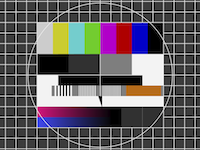
\includegraphics[height=0.9\textheight, width=\linewidth, keepaspectratio]{Images/test_pattern.png}%\caption{C Amsler, T DeGrand et al 2017 - Quark Model.jpg}
      \figcite{C.Amsler.2017}
    
    \end{frame}


    
    % Bibliography    
  \begin{frame}[allowframebreaks, noframenumbering, plain]{Literaturverzeichnis}
   \printbibliography%[nottype=unpublished]
    \end{frame}

\end{document}
